\documentclass[tikz, border=1mm]{standalone}
\usetikzlibrary{arrows, shapes.gates.logic.US, calc}
\begin{document}
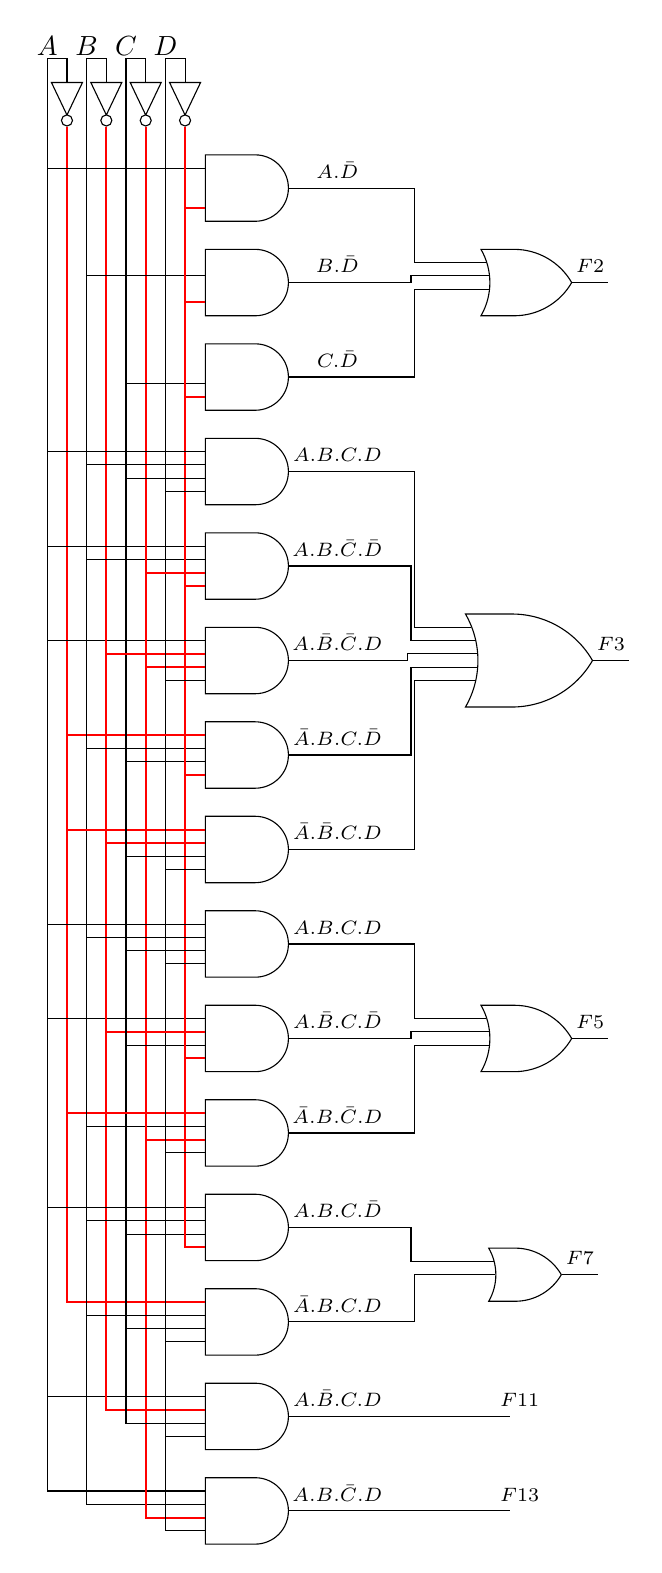
\begin{tikzpicture}

 %%Paramaters
%% var position, can be modified
\def\varPos{19.80}
\def\FunctionPos{6}
\node (x) at (0, \varPos) {$A$};
\node (y) at (0.5, \varPos) {$B$};
\node (z) at (1, \varPos) {$C$};
\node (w) at (1.5, \varPos) {$D$};

                \node[not gate US, draw, rotate=270] at ($(x) + (0.25, -0.6)$) (notx) {};
                \draw ($(x)+(0,-1ex)$) -| (notx.input); 
                \node[not gate US, draw, rotate=270] at ($(y) + (0.25, -0.6)$) (noty) {};
                \draw ($(y)+(0,-1ex)$) -| (noty.input); 
                \node[not gate US, draw, rotate=270] at ($(z) + (0.25, -0.6)$) (notz) {};
                \draw ($(z)+(0,-1ex)$) -| (notz.input);
                \node[not gate US, draw, rotate=270] at ($(w) + (0.25, -0.6)$) (notw) {};
                \draw ($(w)+(0,-1ex)$) -| (notw.input);
             

 %% ***Function F13 : Gate for term n° 1 [ A.B.C'.D ]***
  
\node[and gate US, draw, rotate=0, logic gate inputs=nnnn] at (2.5, 1.20) (xandy1) {};\draw (xandy1.output) -- node[above]{\scriptsize $ A.B.\bar C.D $} ($(xandy1) + (1.8, 0)$);
                % X
\draw ($(x) + (0, -1ex)$)|- (xandy1.input 1);
% Y
\draw ($(y) + (0, -1ex)$)|- (xandy1.input 2);
% Z
\draw [line width=0.25mm,   red] (notz.output)
            -- ([xshift=0cm]notz.output) |- (xandy1.input 3);
% W
\draw ($(w) + (0, -1ex)$)|- (xandy1.input 4);


%% Function F13 Large OR Gate

\node at (\FunctionPos, 1.20) (xory1) {};


            \draw (xory1) node[above]{\scriptsize $F13$} ($(xory1.east) + (+3ex, 0)$);


            \draw (xandy1.output) -- ([xshift=1.60cm]xandy1.output) |- (xory1);

 

 %% ***Function F11 : Gate for term n° 1 [ A.B'.C.D ]***
  
                \node[and gate US, draw, rotate=0, logic gate inputs=nnnn] at (2.5, 2.40) (xandy2) {};\draw (xandy2.output) -- node[above]{\scriptsize $ A.\bar B.C.D $} ($(xandy2) + (1.8, 0)$);
                % X
\draw ($(x) + (0, -1ex)$)|- (xandy2.input 1);
% Y
\draw [line width=0.25mm,   red] (noty.output)
            -- ([xshift=0cm]noty.output) |- (xandy2.input 2);
% Z
\draw ($(z) + (0, -1ex)$)|- (xandy2.input 3);
% W
\draw ($(w) + (0, -1ex)$)|- (xandy2.input 4);


%% Function F11 Large OR Gate

\node at (\FunctionPos, 2.40) (xory2) {};


            \draw (xory2) node[above]{\scriptsize $F11$} ($(xory2.east) + (+3ex, 0)$);


            \draw (xandy2.output) -- ([xshift=1.60cm]xandy2.output) |- (xory2);

 

 %% ***Function F7 : Gate for term n° 1 [ A'.B.C.D ]***
  
                \node[and gate US, draw, rotate=0, logic gate inputs=nnnn] at (2.5, 3.60) (xandy3) {};\draw (xandy3.output) -- node[above]{\scriptsize $ \bar A.B.C.D $} ($(xandy3) + (1.8, 0)$);
                % X
\draw [line width=0.25mm,   red] (notx.output)
            -- ([xshift=0cm]notx.output) |- (xandy3.input 1);
% Y
\draw ($(y) + (0, -1ex)$)|- (xandy3.input 2);
% Z
\draw ($(z) + (0, -1ex)$)|- (xandy3.input 3);
% W
\draw ($(w) + (0, -1ex)$)|- (xandy3.input 4);
 

 %% ***Function F7 : Gate for term n° 2 [ A.B.C.D' ]***
  
                \node[and gate US, draw, rotate=0, logic gate inputs=nnnn] at (2.5, 4.80) (xandy4) {};\draw (xandy4.output) -- node[above]{\scriptsize $ A.B.C.\bar D $} ($(xandy4) + (1.8, 0)$);
                % X
\draw ($(x) + (0, -1ex)$)|- (xandy4.input 1);
% Y
\draw ($(y) + (0, -1ex)$)|- (xandy4.input 2);
% Z
\draw ($(z) + (0, -1ex)$)|- (xandy4.input 3);
% W
\draw [line width=0.25mm,   red] (notw.output)
            -- ([xshift=0cm]notw.output) |- (xandy4.input 4);


%% Function F7 Large OR Gate

\node[or gate US, draw, rotate=0, logic gate inputs=nnn] at (\FunctionPos, 4.20) (xory3) {};


            \draw (xory3.output) -- node[above]{\scriptsize $F7$} ($(xory3.east) + (+3ex, 0)$);


            \draw (xandy3.output) -- ([xshift=1.60cm]xandy3.output) |- (xory3.input 2);

\draw (xandy4.output) -- ([xshift=1.55cm]xandy4.output) |- (xory3.input 1);

 

 %% ***Function F5 : Gate for term n° 1 [ A'.B.C'.D ]***
  
                \node[and gate US, draw, rotate=0, logic gate inputs=nnnn] at (2.5, 6.00) (xandy5) {};\draw (xandy5.output) -- node[above]{\scriptsize $ \bar A.B.\bar C.D $} ($(xandy5) + (1.8, 0)$);
                % X
\draw [line width=0.25mm,   red] (notx.output)
            -- ([xshift=0cm]notx.output) |- (xandy5.input 1);
% Y
\draw ($(y) + (0, -1ex)$)|- (xandy5.input 2);
% Z
\draw [line width=0.25mm,   red] (notz.output)
            -- ([xshift=0cm]notz.output) |- (xandy5.input 3);
% W
\draw ($(w) + (0, -1ex)$)|- (xandy5.input 4);
 

 %% ***Function F5 : Gate for term n° 2 [ A.B'.C.D' ]***
  
                \node[and gate US, draw, rotate=0, logic gate inputs=nnnn] at (2.5, 7.20) (xandy6) {};\draw (xandy6.output) -- node[above]{\scriptsize $ A.\bar B.C.\bar D $} ($(xandy6) + (1.8, 0)$);
                % X
\draw ($(x) + (0, -1ex)$)|- (xandy6.input 1);
% Y
\draw [line width=0.25mm,   red] (noty.output)
            -- ([xshift=0cm]noty.output) |- (xandy6.input 2);
% Z
\draw ($(z) + (0, -1ex)$)|- (xandy6.input 3);
% W
\draw [line width=0.25mm,   red] (notw.output)
            -- ([xshift=0cm]notw.output) |- (xandy6.input 4);
 

 %% ***Function F5 : Gate for term n° 3 [ A.B.C.D ]***
  
                \node[and gate US, draw, rotate=0, logic gate inputs=nnnn] at (2.5, 8.40) (xandy7) {};\draw (xandy7.output) -- node[above]{\scriptsize $ A.B.C.D $} ($(xandy7) + (1.8, 0)$);
                % X
\draw ($(x) + (0, -1ex)$)|- (xandy7.input 1);
% Y
\draw ($(y) + (0, -1ex)$)|- (xandy7.input 2);
% Z
\draw ($(z) + (0, -1ex)$)|- (xandy7.input 3);
% W
\draw ($(w) + (0, -1ex)$)|- (xandy7.input 4);


%% Function F5 Large OR Gate

\node[or gate US, draw, rotate=0, logic gate inputs=nnnn] at (\FunctionPos, 7.20) (xory5) {};


            \draw (xory5.output) -- node[above]{\scriptsize $F5$} ($(xory5.east) + (+3ex, 0)$);


            \draw (xandy5.output) -- ([xshift=1.60cm]xandy5.output) |- (xory5.input 3);

\draw (xandy6.output) -- ([xshift=1.55cm]xandy6.output) |- (xory5.input 2);

\draw (xandy7.output) -- ([xshift=1.60cm]xandy7.output) |- (xory5.input 1);

 

 %% ***Function F3 : Gate for term n° 1 [ A'.B'.C.D ]***
  
                \node[and gate US, draw, rotate=0, logic gate inputs=nnnn] at (2.5, 9.60) (xandy8) {};\draw (xandy8.output) -- node[above]{\scriptsize $ \bar A.\bar B.C.D $} ($(xandy8) + (1.8, 0)$);
                % X
\draw [line width=0.25mm,   red] (notx.output)
            -- ([xshift=0cm]notx.output) |- (xandy8.input 1);
% Y
\draw [line width=0.25mm,   red] (noty.output)
            -- ([xshift=0cm]noty.output) |- (xandy8.input 2);
% Z
\draw ($(z) + (0, -1ex)$)|- (xandy8.input 3);
% W
\draw ($(w) + (0, -1ex)$)|- (xandy8.input 4);
 

 %% ***Function F3 : Gate for term n° 2 [ A'.B.C.D' ]***
  
                \node[and gate US, draw, rotate=0, logic gate inputs=nnnn] at (2.5, 10.80) (xandy9) {};\draw (xandy9.output) -- node[above]{\scriptsize $ \bar A.B.C.\bar D $} ($(xandy9) + (1.8, 0)$);
                % X
\draw [line width=0.25mm,   red] (notx.output)
            -- ([xshift=0cm]notx.output) |- (xandy9.input 1);
% Y
\draw ($(y) + (0, -1ex)$)|- (xandy9.input 2);
% Z
\draw ($(z) + (0, -1ex)$)|- (xandy9.input 3);
% W
\draw [line width=0.25mm,   red] (notw.output)
            -- ([xshift=0cm]notw.output) |- (xandy9.input 4);
 

 %% ***Function F3 : Gate for term n° 3 [ A.B'.C'.D ]***
  
                \node[and gate US, draw, rotate=0, logic gate inputs=nnnn] at (2.5, 12.00) (xandy10) {};\draw (xandy10.output) -- node[above]{\scriptsize $ A.\bar B.\bar C.D $} ($(xandy10) + (1.8, 0)$);
                % X
\draw ($(x) + (0, -1ex)$)|- (xandy10.input 1);
% Y
\draw [line width=0.25mm,   red] (noty.output)
            -- ([xshift=0cm]noty.output) |- (xandy10.input 2);
% Z
\draw [line width=0.25mm,   red] (notz.output)
            -- ([xshift=0cm]notz.output) |- (xandy10.input 3);
% W
\draw ($(w) + (0, -1ex)$)|- (xandy10.input 4);
 

 %% ***Function F3 : Gate for term n° 4 [ A.B.C'.D' ]***
  
                \node[and gate US, draw, rotate=0, logic gate inputs=nnnn] at (2.5, 13.20) (xandy11) {};\draw (xandy11.output) -- node[above]{\scriptsize $ A.B.\bar C.\bar D $} ($(xandy11) + (1.8, 0)$);
                % X
\draw ($(x) + (0, -1ex)$)|- (xandy11.input 1);
% Y
\draw ($(y) + (0, -1ex)$)|- (xandy11.input 2);
% Z
\draw [line width=0.25mm,   red] (notz.output)
            -- ([xshift=0cm]notz.output) |- (xandy11.input 3);
% W
\draw [line width=0.25mm,   red] (notw.output)
            -- ([xshift=0cm]notw.output) |- (xandy11.input 4);
 

 %% ***Function F3 : Gate for term n° 5 [ A.B.C.D ]***
  
                \node[and gate US, draw, rotate=0, logic gate inputs=nnnn] at (2.5, 14.40) (xandy12) {};\draw (xandy12.output) -- node[above]{\scriptsize $ A.B.C.D $} ($(xandy12) + (1.8, 0)$);
                % X
\draw ($(x) + (0, -1ex)$)|- (xandy12.input 1);
% Y
\draw ($(y) + (0, -1ex)$)|- (xandy12.input 2);
% Z
\draw ($(z) + (0, -1ex)$)|- (xandy12.input 3);
% W
\draw ($(w) + (0, -1ex)$)|- (xandy12.input 4);


%% Function F3 Large OR Gate

\node[or gate US, draw, rotate=0, logic gate inputs=nnnnnn] at (\FunctionPos, 12.00) (xory8) {};


            \draw (xory8.output) -- node[above]{\scriptsize $F3$} ($(xory8.east) + (+3ex, 0)$);


            \draw (xandy8.output) -- ([xshift=1.60cm]xandy8.output) |- (xory8.input 5);

\draw (xandy9.output) -- ([xshift=1.55cm]xandy9.output) |- (xory8.input 4);

\draw (xandy10.output) -- ([xshift=1.50cm]xandy10.output) |- (xory8.input 3);

\draw (xandy11.output) -- ([xshift=1.55cm]xandy11.output) |- (xory8.input 2);

\draw (xandy12.output) -- ([xshift=1.60cm]xandy12.output) |- (xory8.input 1);

 

 %% ***Function F2 : Gate for term n° 1 [ C.D' ]***
  
                \node[and gate US, draw, rotate=0, logic gate inputs=nnnn] at (2.5, 15.60) (xandy13) {};\draw (xandy13.output) -- node[above]{\scriptsize $ C.\bar D $} ($(xandy13) + (1.8, 0)$);
                % Z
\draw ($(z) + (0, -1ex)$)|- (xandy13.input 3);
% W
\draw [line width=0.25mm,   red] (notw.output)
            -- ([xshift=0cm]notw.output) |- (xandy13.input 4);
 

 %% ***Function F2 : Gate for term n° 2 [ B.D' ]***
  
                \node[and gate US, draw, rotate=0, logic gate inputs=nnnn] at (2.5, 16.80) (xandy14) {};\draw (xandy14.output) -- node[above]{\scriptsize $ B.\bar D $} ($(xandy14) + (1.8, 0)$);
                % Y
\draw ($(y) + (0, -1ex)$)|- (xandy14.input 2);
% W
\draw [line width=0.25mm,   red] (notw.output)
            -- ([xshift=0cm]notw.output) |- (xandy14.input 4);
 

 %% ***Function F2 : Gate for term n° 3 [ A.D' ]***
  
                \node[and gate US, draw, rotate=0, logic gate inputs=nnnn] at (2.5, 18.00) (xandy15) {};\draw (xandy15.output) -- node[above]{\scriptsize $ A.\bar D $} ($(xandy15) + (1.8, 0)$);
                % X
\draw ($(x) + (0, -1ex)$)|- (xandy15.input 1);
% W
\draw [line width=0.25mm,   red] (notw.output)
            -- ([xshift=0cm]notw.output) |- (xandy15.input 4);


%% Function F2 Large OR Gate

\node[or gate US, draw, rotate=0, logic gate inputs=nnnn] at (\FunctionPos, 16.80) (xory13) {};


            \draw (xory13.output) -- node[above]{\scriptsize $F2$} ($(xory13.east) + (+3ex, 0)$);


            \draw (xandy13.output) -- ([xshift=1.60cm]xandy13.output) |- (xory13.input 3);

\draw (xandy14.output) -- ([xshift=1.55cm]xandy14.output) |- (xory13.input 2);

\draw (xandy15.output) -- ([xshift=1.60cm]xandy15.output) |- (xory13.input 1);

 \end{tikzpicture}
         \end{document}
